\documentclass[a4paper,12pt]{scrartcl}
\usepackage{amsmath}
\usepackage{amsfonts}
\usepackage{amssymb}

\usepackage[latin1]{inputenc}
\usepackage[T1]{fontenc}
\usepackage[pdftex]{graphicx}

\usepackage{url}
\usepackage{vmargin} 

\setpapersize{A4}
\setmargins{3.5cm}
					 {1.5cm}
           {14.7cm}
           {23.42cm}
           {14pt}
           {1cm}
           {0pt}
           {2cm}         
\renewcommand{\floatpagefraction}{0.7} 

\usepackage{ccaption}

\setlength{\abovecaptionskip}{0mm} 


\usepackage{scrpage2} 
\renewcommand{\headfont}{\footnotesize\sffamily} 
\renewcommand{\pnumfont}{\footnotesize\sffamily}

\defpagestyle{cb}{
(\textwidth,0pt)
{\pagemark\hfill\headmark\hfill}
{\hfill\headmark\hfill\pagemark}
{\hfill\headmark\hfill\pagemark}
(\textwidth,1pt)}
%
{(\textwidth,1pt)
{{\it Quantum Circuit Simulator}\hfill Mert Can �IKLA}
{Mert Can �IKLA\hfill{\it Quantum Circuit Simulator}}
{Mert Can �IKLA\hfill{\it Quantum Circuit Simulator}}
(\textwidth,0pt)
}

\renewpagestyle{plain}
	{(\textwidth,0pt)
		{\hfill}{\hfill}{\hfill}
	(\textwidth,0pt)}
	{(\textwidth,0pt)
		{\hfill}{\hfill}{\hfill}
	(\textwidth,0pt)}

\renewcommand{\footnoterule}{\rule{5cm}{0.2mm} \vspace{0.3cm}} 
\deffootnote[1em]{1em}{1em}{\textsuperscript{\normalfont\thefootnotemark}} 


\pagestyle{plain} 

\begin{document}

\begin{center}

\centering

\\
\vspace{7cm}


{\Huge \textbf{Quantum Circuit Simulator}}
\noindent\rule{15cm}{0.4pt}\\
\vspace{0.6cm}
{\LARGE Software Design Documentation\\ \vspace{0.4cm}
SE 360 Advances In Software Development}
\vspace{5cm}

{\Large\bf\sf Mert Can �IKLA}
\vspace{5cm}

{\Large\bf\sf November 29, 2013}

\vspace{\fill}

\end{center}
\newpage

\pagestyle{cb} 

\tableofcontents

\newpage

\section{Introduction}
\setlength{\parindent}{25pt}
\indent
\hspace{1cm}Quantum Circuit Simulator is an application for Android capable of simulating essential gates used in fields of quantum computation and quantum information processing. The application aims to provide a way to simulate and see how a quantum calculation actually takes place.
 
\subsection{Goals and Objectives }

\subsubsection{Ease of Use}
\hspace{1cm}First of all application is fairly easy to use with a clean and simple GUI. Drag/drop
which is an intuitive action on a touch screen will be implemented with the framework
included in Android API 11.
\subsubsection{Functionality}
\hspace{1cm}This project will be able to simulate behaviour of any quantum gate or circuit that acts
on up to 8 qubits or possibly less depending on screen resolution of the device running.
\subsubsection{Speed}
\hspace{1cm}This application which has matrix multiplications which is a heavy calculation at its core, 
will be able to run smootly on any mobile device.
\subsection{Target Users and Devices}
\hspace{1cm}Students studying mathematics, physics or computer engineering is the main targeted user
group of this application however it might be a useful tool for researchers and professionals
aswell. Mobile devices that are running Android 3.0 or above such as tablets or cellphones with a
screen larger than 5 inches are the targeted devices of this project.

\newpage
\section{User Interface}

\begin{figure}[!ht]
\centering
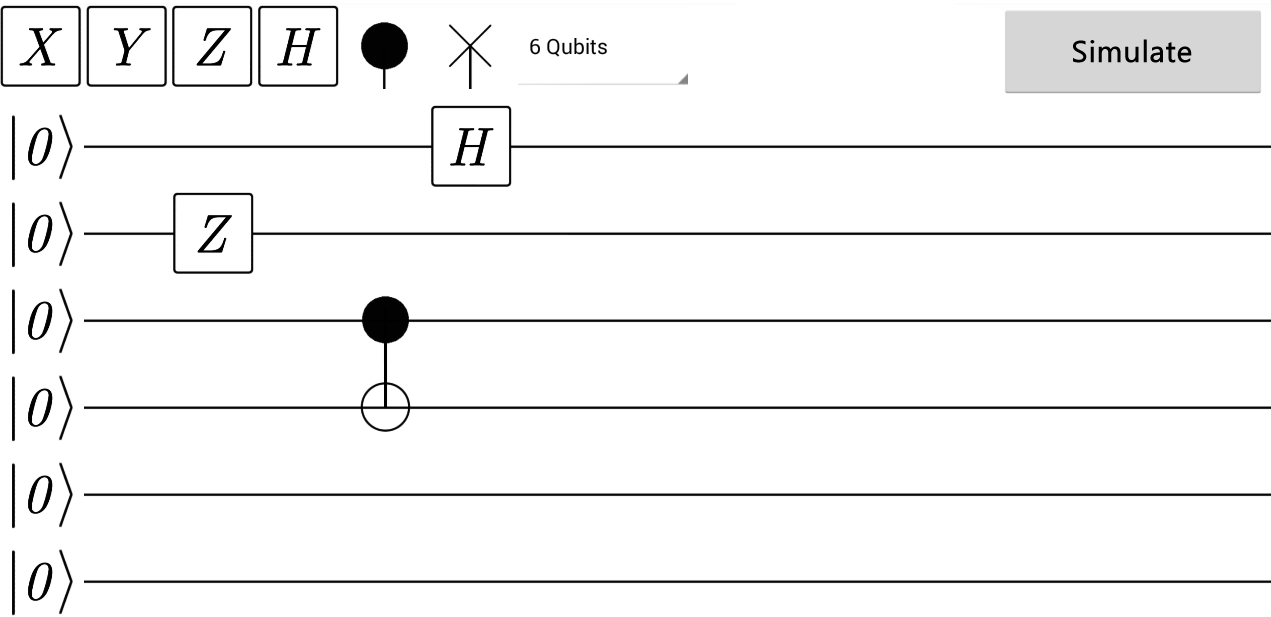
\includegraphics[width=\textwidth]{ss2}
\caption{Sample User Interface}
\end{figure}

The user interface will be featured in fullscreen mode and defined in a single XML file. There is a single screen to be displayed with a result window popping up after simulation. 

\subsection{Toolbar}
\begin{figure}[!ht]
\centering
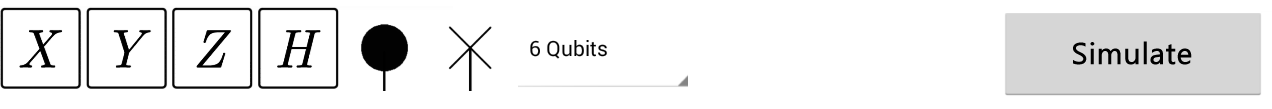
\includegraphics[width=\textwidth]{topBar}
\caption{Sample Toolbar}
\end{figure}


The toolbar is to be defined as a horizontal LinearLayout object specified by the Android API. The toolbar holds quantum gates, spinner for number of qubit selection and the simulate button. A sample is shown in Figure 2.

\begin{figure}[!ht]
\centering
 
\includegraphics[scale=0.50]{x}
\caption{Sample Gate Representation for Pauli-X}
\end{figure}

Quantum gates will be represented as shown which is the universal standard. This is represented by the class QuantumGate which is an extension of the android class ImageView that makes a copy of itself at start of a drag operation when it is the source, or can be used as a target of the drop operation which causes the source object to be deleted.  A sample is shown in Figure 3.
\newpage
The spinner object will display an array of text objects that on click sets the activeQbits to the corresponding value, activeQbits determine the number of qButton and gateContainer objects on the circuit board. 
\begin{figure}[!ht]
\centering
 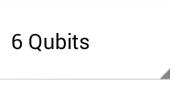
\includegraphics[scale=0.50]{qubitselect}
\caption{Spinner for number of qubit selection}
\end{figure}



\subsection{Circuit Board}

\begin{figure}[!ht]
\centering
 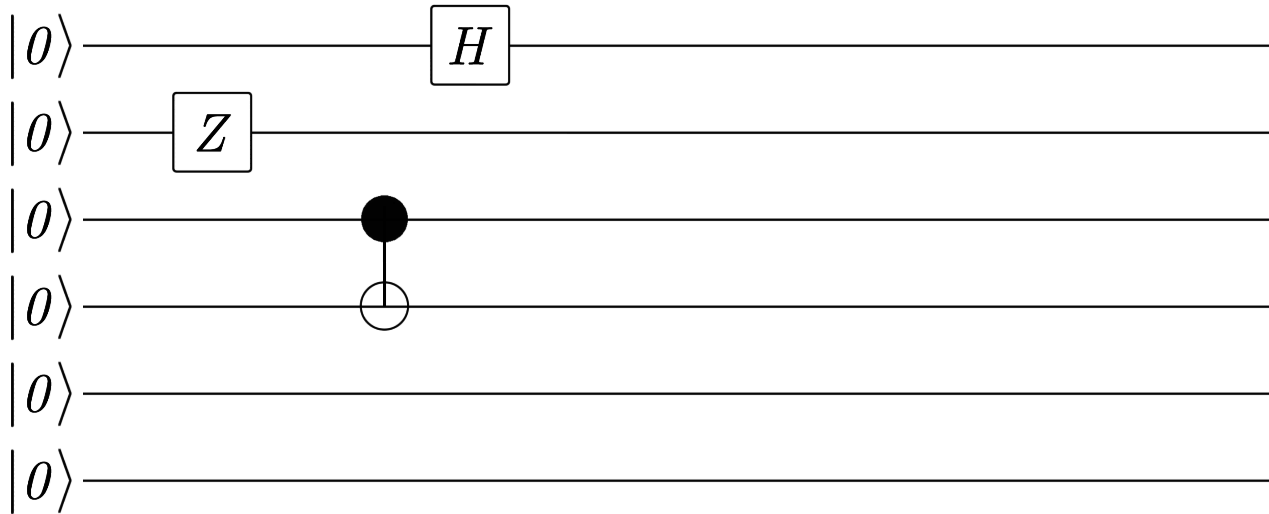
\includegraphics[width=\textwidth]{workbench}
\caption{Sample Circuit Board}
\end{figure}
The circuit board is comprised of the buttons on the left and equal number of horizontally structured GateContainer objects.\\
\begin{figure}[!ht]
\centering
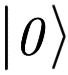
\includegraphics[scale=0.50]{qbut}
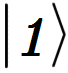
\includegraphics[scale=0.50]{qbut2}
\caption{Buttons to change the initial state of a qubit.}
\end{figure}

Buttons will change between the initial states 0 and 1 on click. GateContainers act as container for QuantumGates initially filled w ith invisible objects to be used as drop target locations.
\newpage
\subsection{Result Screen}
The result screen is drawn by the simulate method. The method will also pass the  The layout is to be defined in a seperate XML file that consists of a single ListView object. 
\begin{figure}[!ht]
\centering
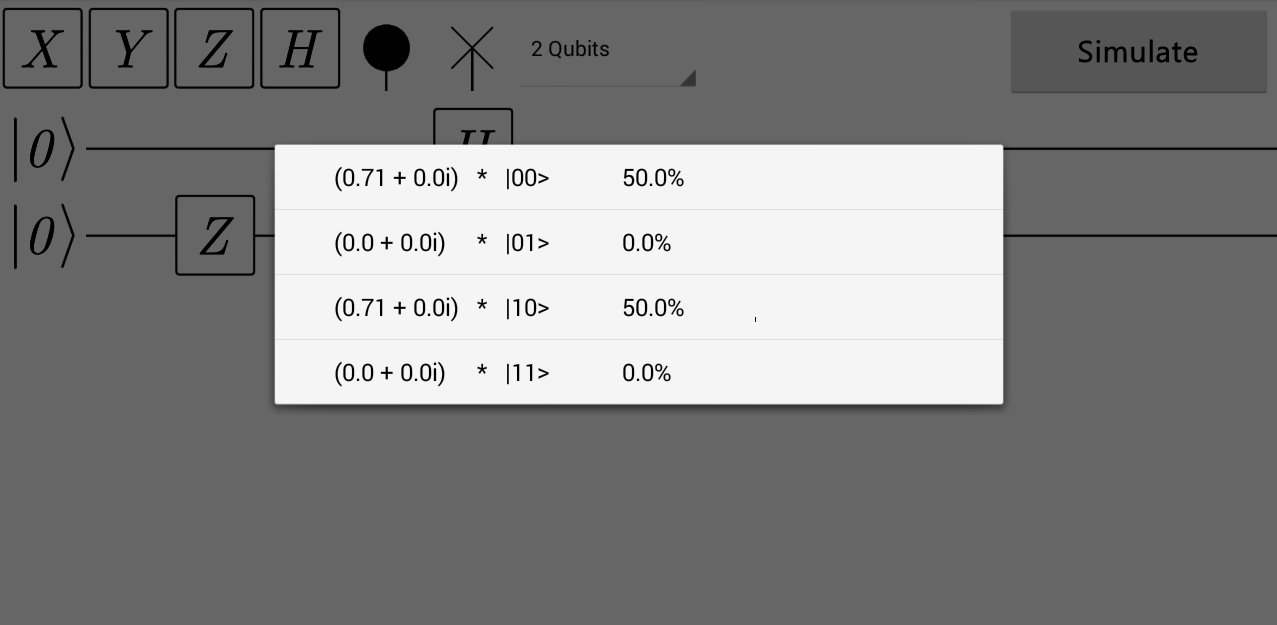
\includegraphics[width=\textwidth]{ss1}
\caption{Example result screen for 2 qubits}
\end{figure}

\newpage

\section{Drag/Drop}
Drag/Drop functionality is to be provided using the framework within Android API. The MainProgram implements interfaces for Touch and Drag Listeners.
\subsection{onDrag}
The onDrag method is called when a draggable object is dropped. The Method identifies the target and source location of the object and what is the base class of object is. Possible actions are explained on Figure 8. 
\begin{figure}[!ht]
\centering
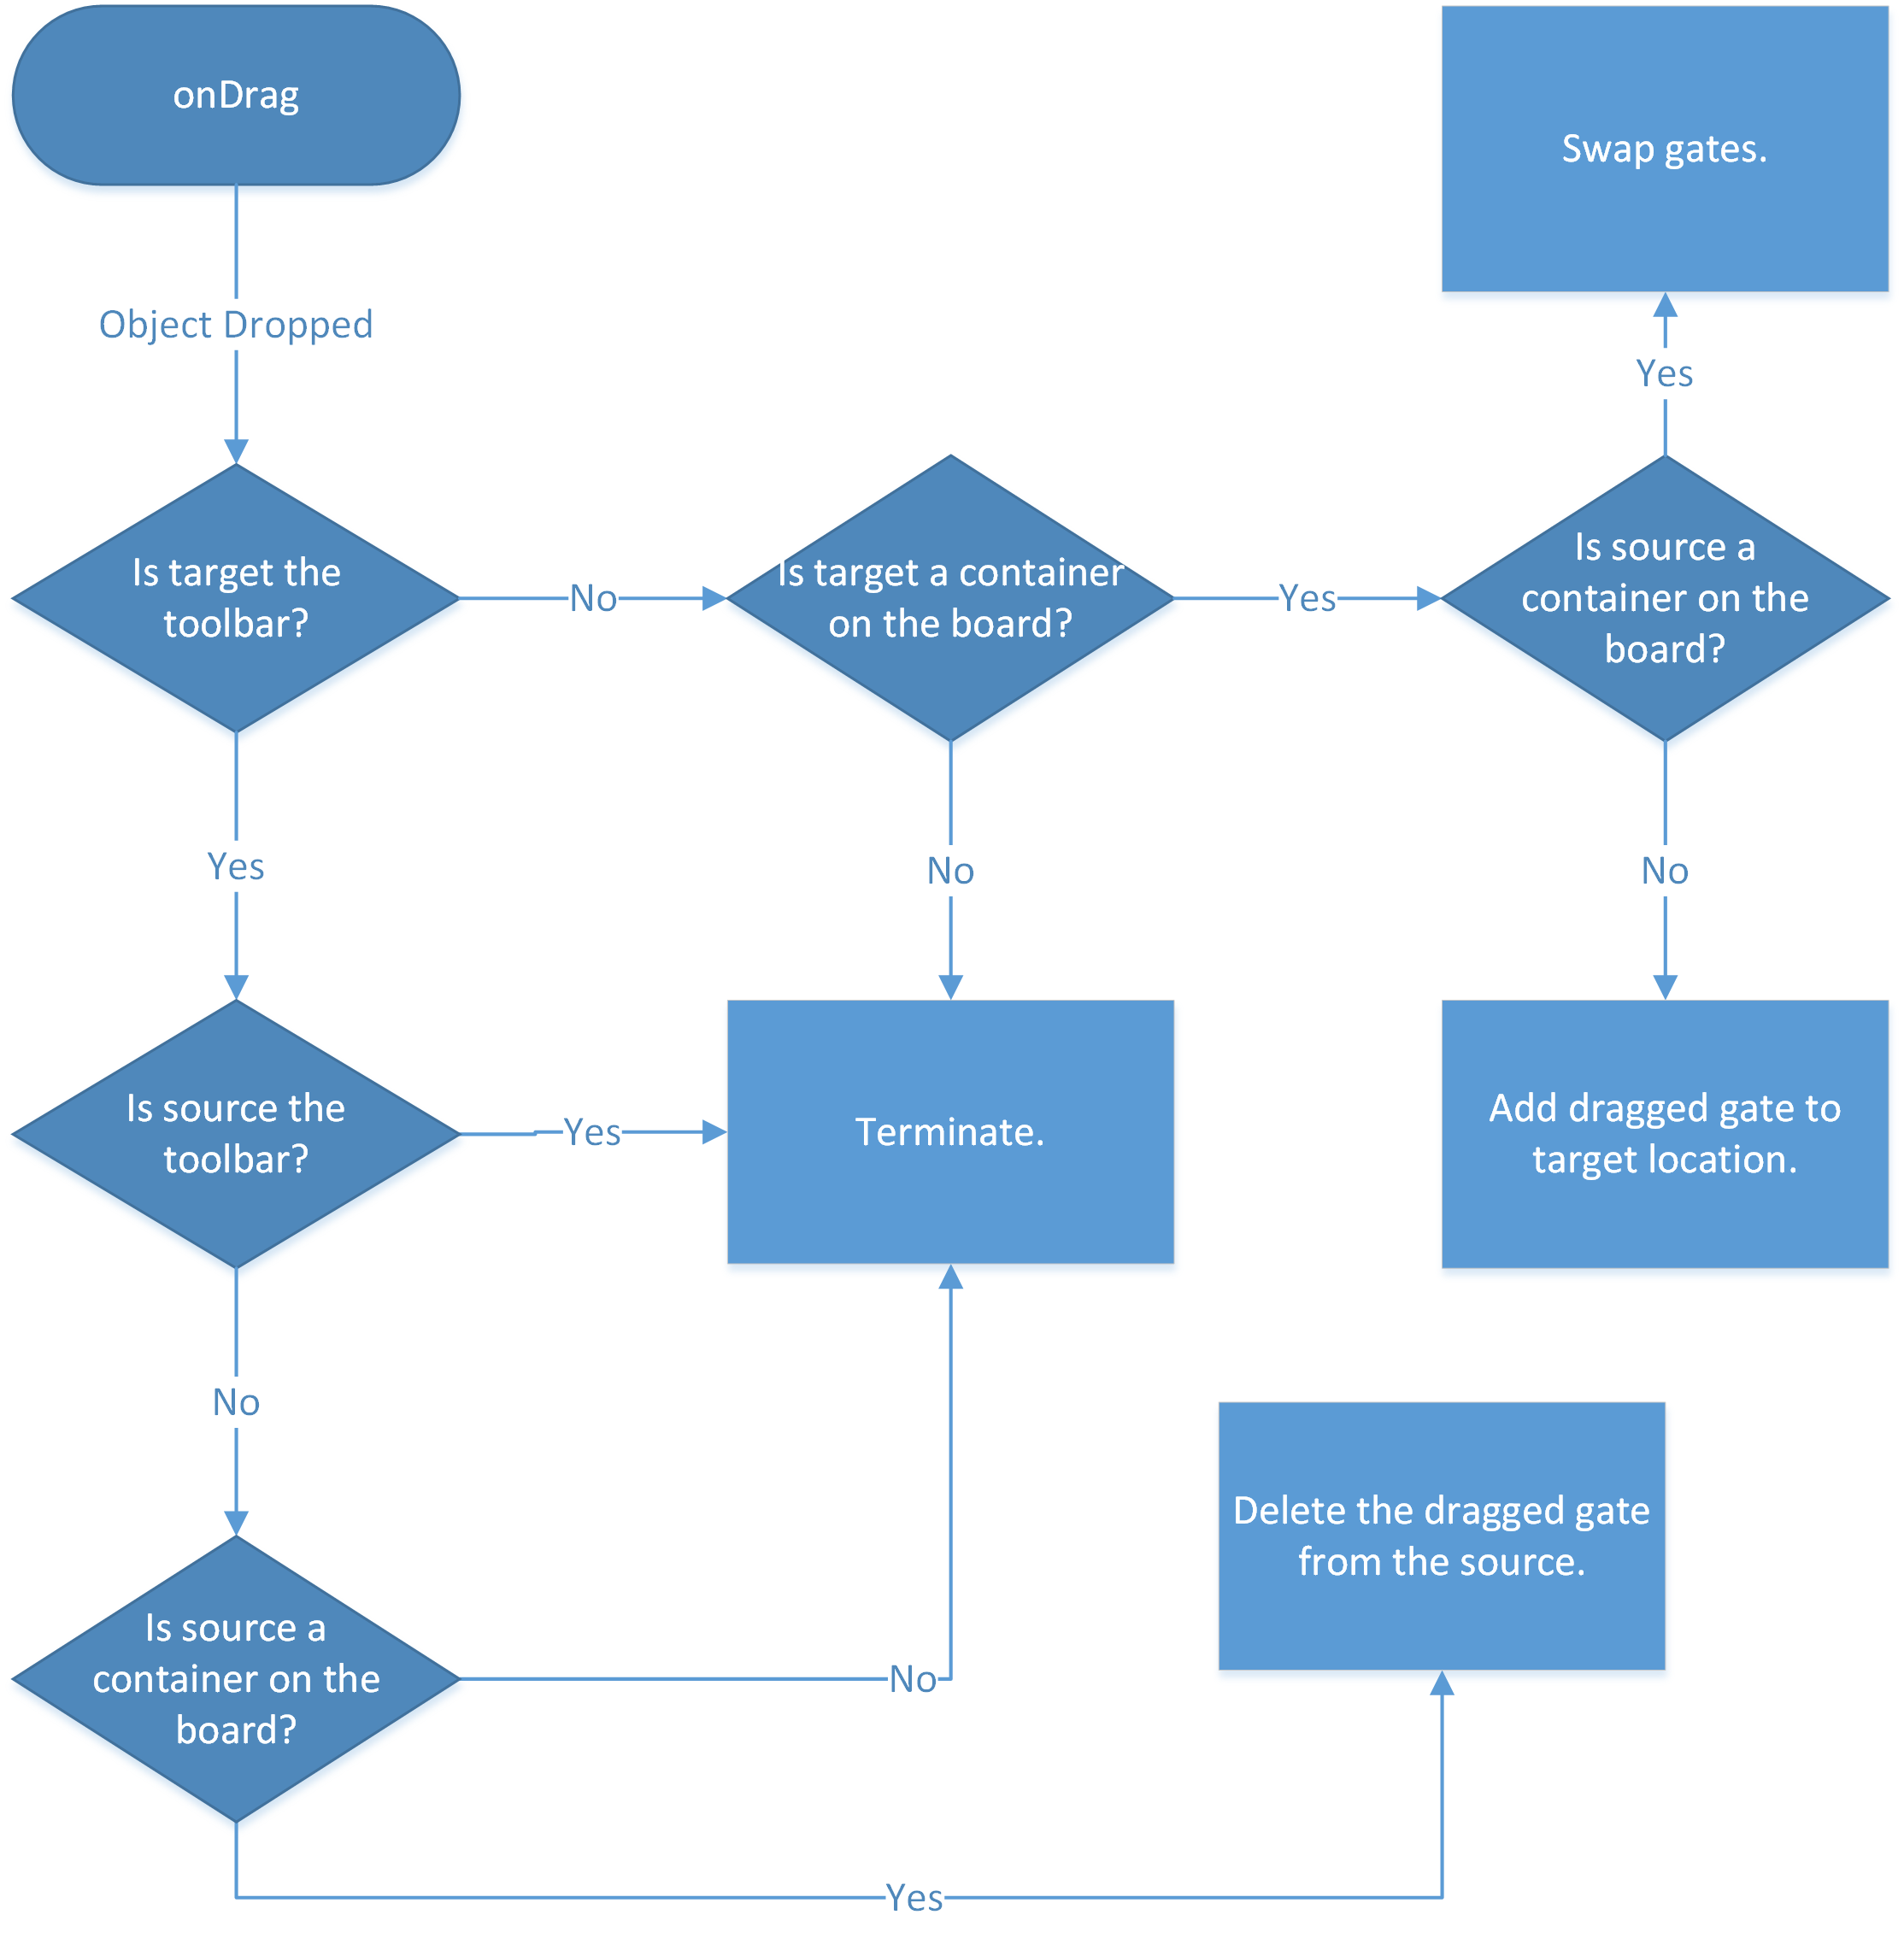
\includegraphics[width=\textwidth]{onDrag}
\caption{Decision diagram for all drag events.}
\end{figure}

\newpage
\section{Class Descriptions}
Classes PauliX, PauliY, PauliZ, Hadamard, Swap and Cnot are simple class representations of the gates. QuBit data values must be set at initialization as well as the gate image resources.
\subsection {UML Diagram}
\begin{figure}[!ht]
\centering
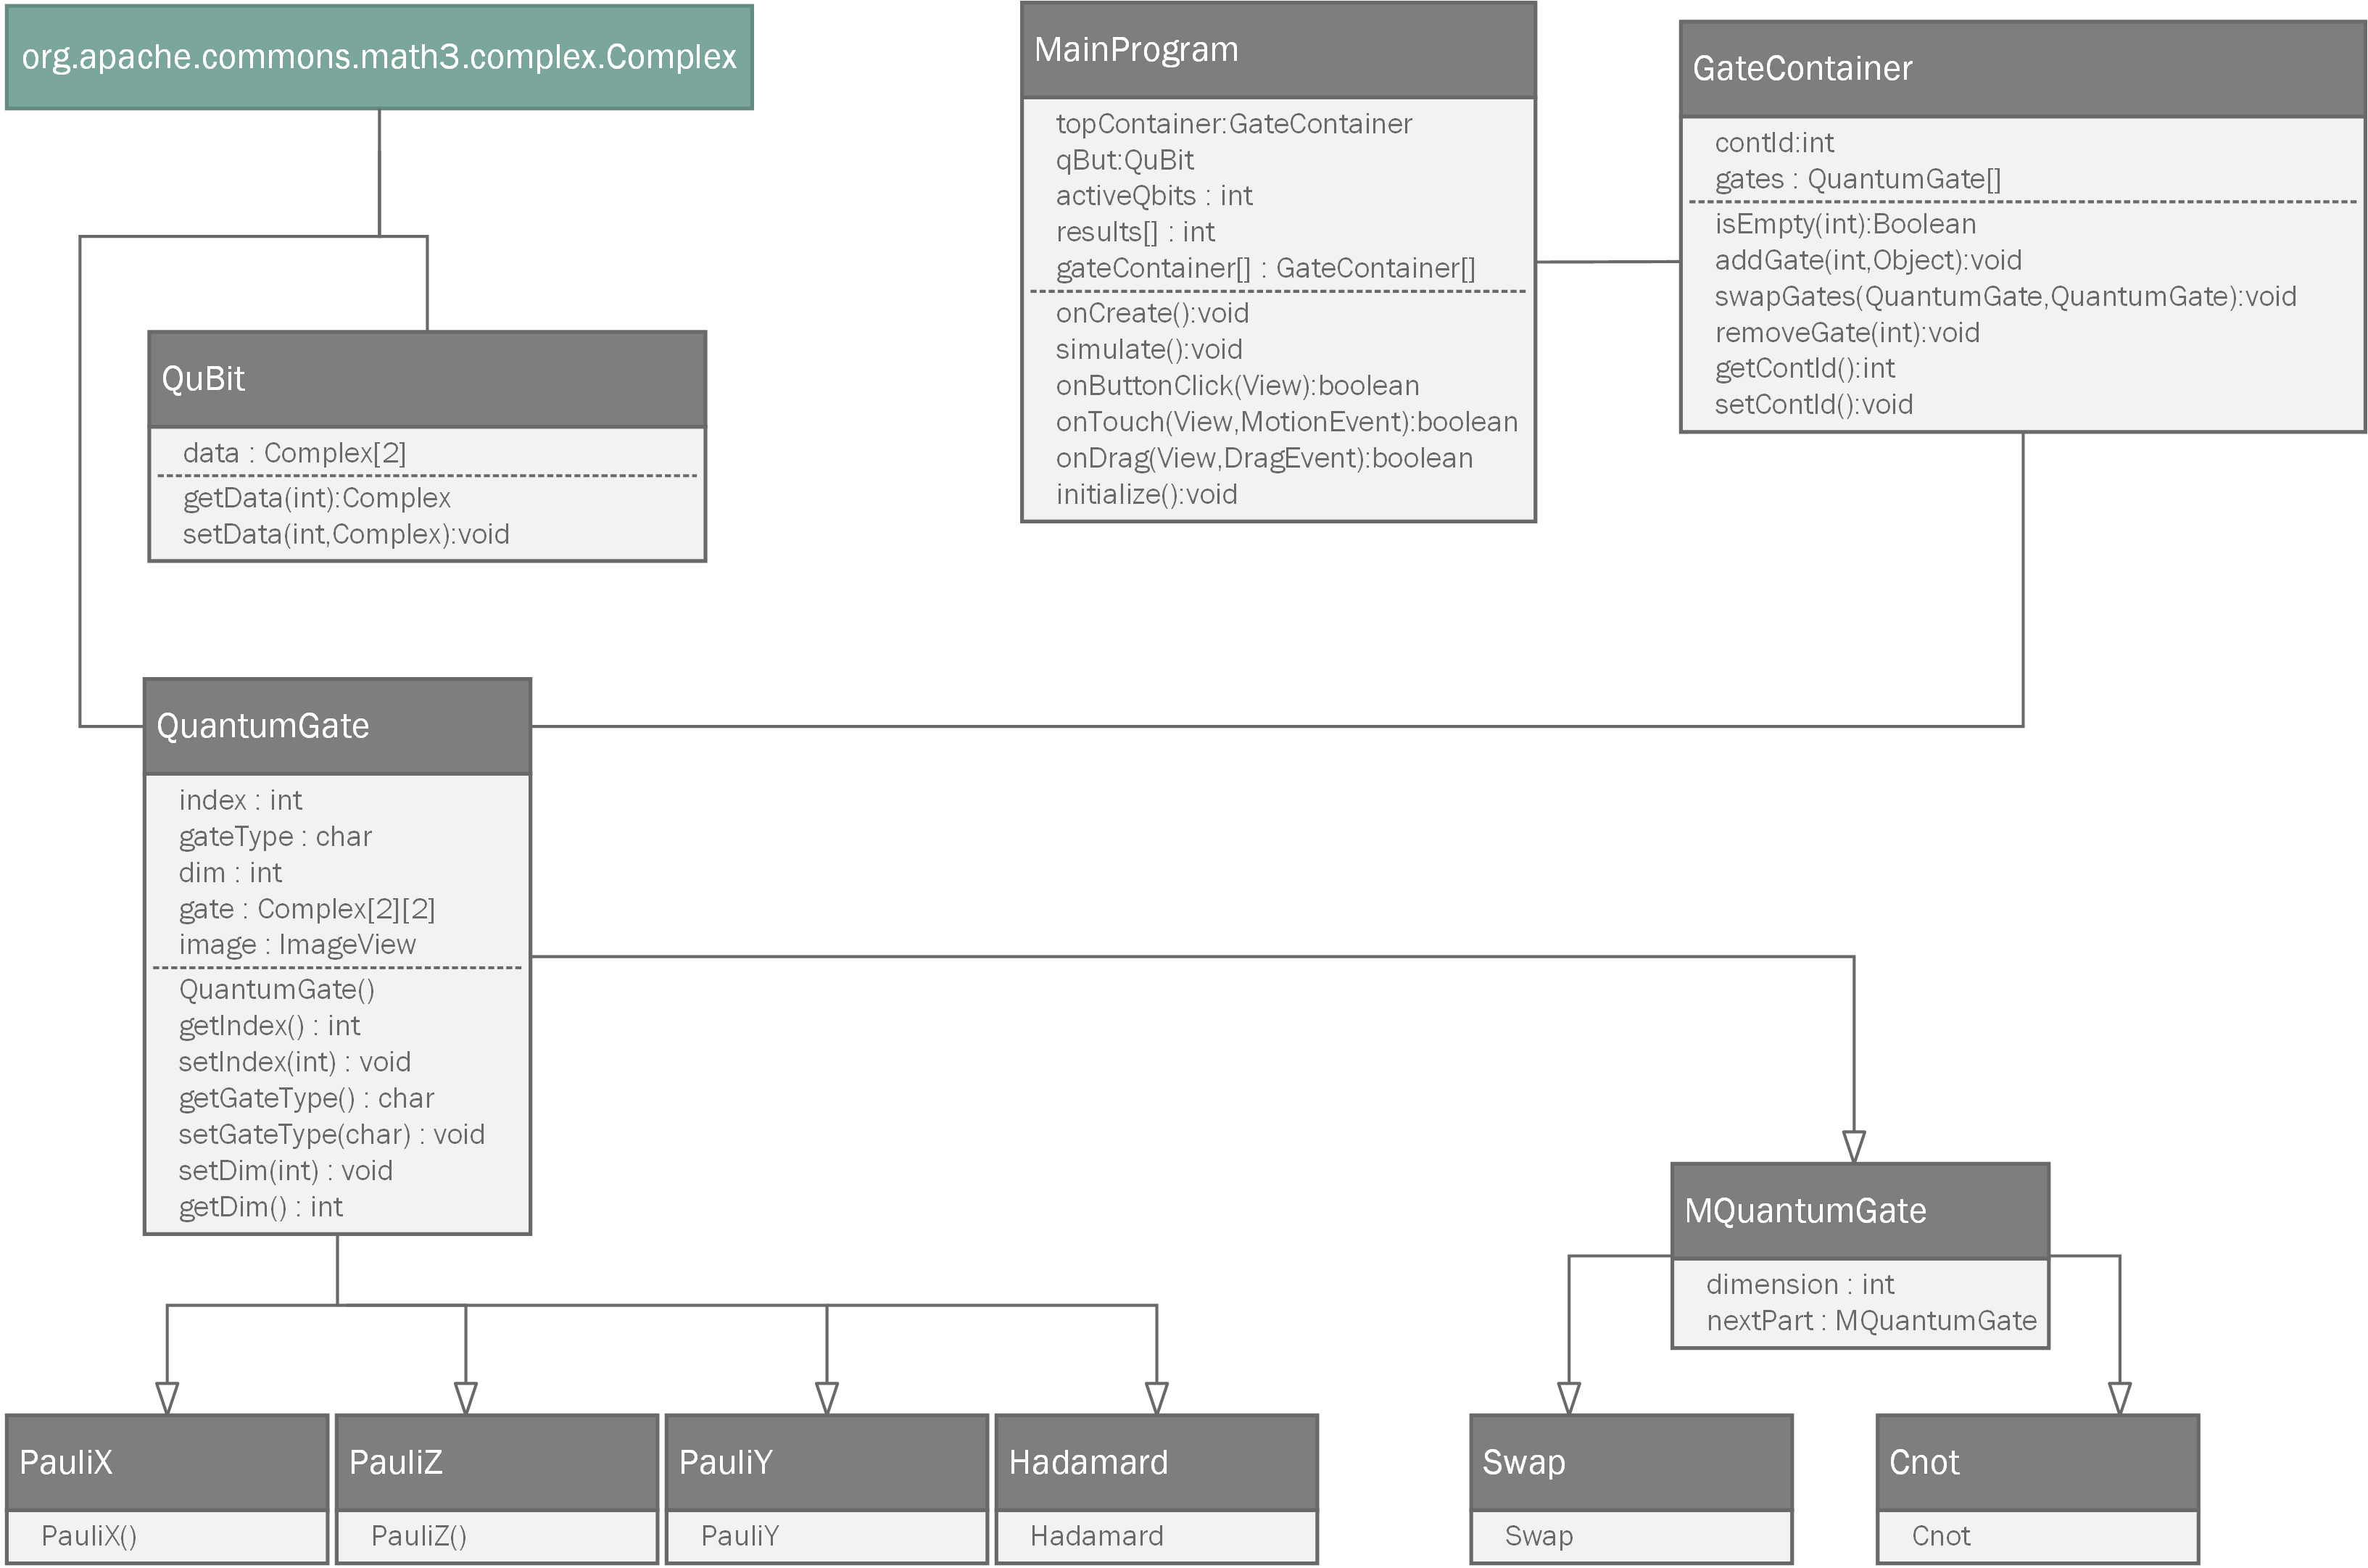
\includegraphics[width=\textwidth]{uml1}
\end{figure}
\newpage
\subsection {MainProgram}
MainProgram is an object with base class Activity and it is executed at startup automatically by Android. 
\paragraph{Attributes}
\begin{itemize}

\item \textbf{topContainer : GateContainer}
\newline
Container shown in toolbar which holds all the QuantumGates Pauli-X, Pauli-Y, Pauli-Z, Hadamard, Swap and Cnot. Any child object within must call setOnTouchListener() and setOnDragListener() methods. On drag events, this object is copied for the drag handler to use as reference. 
\item \textbf{qButton : QuBit}
\newline
QuBit object that start with initial value 0 and corresponding image of $\vert 0  \rangle$ can change to $\vert 1  \rangle$ on click. This object is setup within XML and calls onButtonClick method by android:onClick attribute set within XML. 
\item \textbf{activeQbits : int}
\newline
activeQbits is set to 1 as default and determines the visible qButton and gateContainer objects.
\item \textbf{results[ ] : ListView}
\newline
This object is filled with TextView populated from the simulate() method. $2^N$ TextView objects are required for N=activeQubits.
\item \textbf{gateContainer : GateContainer[20]} 
\newline
Container initially filled with invisible QuantumGates that fits the screen.  Drag/Drop unto this area is valid. Array size of this object is determined by activeQbits. 20 should be sufficient to fill the screen on any resolution.
\end{itemize}
\paragraph{Methods}
\begin{itemize}

\item \textbf{onCreate() : void}
\newline
This method is called only by Android at startup. Any initilization and layout drawings are done in this method. Setting up event listeners is also handled here. 
\item \textbf{simulate() : void}
\newline
Calculates the state of each qubit by iterating through the gateContainer. At each step data attribute of corresponding qubit is multiplied with the matrix contained in QuantumGate object's gate matrix. After calculation 
results are added to an array of TextView's and passed to the result screen for display. 
\newpage

\subsection {QuantumGate}

QuantumGate class extends ImageView class and is to be used to display quantum gates and store information about it. 
\paragraph{Attributes}
\begin{itemize}
\item \textbf{index : int}.
\newline
This attribute containes the location index of the gate. Index is initialized to -1 and can have values between 0 and 20, 0 being the first gate in the gateContainer and 20 last.
\item \textbf{gateType : char}
\newline
This attribute is used to easily identify the gate type of the object. Set to X for Pauli-X, H for Hadamard etc.
\item \textbf{gate : Complex[2][2]}
\newline
Square matrix of size 2 that represents gate as the corresponding unitary matrix. Apache Commons java library for complex numbers is used for storing complex numbers.
\end{itemize}
\paragraph{Methods}
\begin{itemize}
\item \textbf{QuantumGate()}
\newline
Default constructor for the class that initializes values and sets an invisible image for ImageView attribute.
\end{itemize}
\subsection{MQuantumGate}

\paragraph{Attributes}
\begin{itemize}
\item \textbf{dim : int}
\newline
Integer object that holds size for the square matrix. Must be a value of $2^{N}$ for a gate that applies to N qubits.
\item \textbf{nextPart : MQuantumGate}
\newline
Holds a reference to the bottom half of a 2 qubit gate. This part will be displayed on the gateContainer under the the one holding the main part with same index. 
\paragraph{Methods}
\end{itemize}
\newpage
\subsection {QuBit}

\paragraph{Attributes}
\begin{itemize}
\item \textbf{data : Complex[2]}.
\newline
Stores vector information for the corresponding qubit.
\end{itemize}

\paragraph{Methods}
\begin{itemize}
\item \textbf{QuBit()}
\newline
Initializes data attribute to 0 with array size 2.
\end{itemize}
\subsection {GateContainer}

\paragraph{Attributes}
\begin{itemize}
\item \textbf{contId : int}
\newline
Identifies the vertical index of gateContainer. Takes values between 0 and 8, 0 for top and 8 for the bottom.
\item \textbf{gates : QuantumGate[20]}
\newline
Holds quantum gate objects to display.	 
\end{itemize}
\paragraph{Methods}
\begin{itemize}

\item \textbf{isEmpty(index) : Boolean}
\newline
This method returns false if this gateContainer does not have a child at position index. True if a QuantumGate object is stored.
\item \textbf{addGate(index,Object) : void}
\newline
Adds the given object to the position index of this gateContainer.
\item \textbf{swapGates(QuantumGate,QuantumGate) : void}
\newline 
Swaps the gates using a temporary QuantumGate object.

\item \textbf{removeGate(int) : void}
\newline
Removes the gate from the given index. Creates a new QuantumGate with no image resource with on drag listener to enable gates to be dropped and added later on.
\end{itemize}

\end{document}



